\documentclass[../../main]{subfiles}
\begin{document}



\section[Bearing and Caster Wheel Design]{Design and Optimization of Bearing and Caster\\ Wheels for Enhanced Performance}

Bearing and caster wheels are essential components in industrial and commercial applications, enabling mobility, load distribution, and operational efficiency. These wheels are widely used in material handling equipment, automotive systems, and heavy machinery, where they reduce friction and ensure smooth movement. Their efficiency and durability directly affect productivity, safety, and cost-effectiveness across industries.

Designing effective wheel systems requires careful consideration of several factors, including material selection, load-bearing capacity, environmental resistance, and compliance with industry standards like ISO 3691-4:2020. Common materials, such as AISI 1045 steel for shafts and AISI 52100 chrome steel for bearings, are chosen for their strength, wear resistance, and durability. Environmental conditions, such as moisture, temperature fluctuations, and corrosive elements, also influence material and coating choices.

The design process involves analyzing mechanical constraints like torque, friction, and stress distribution, supported by calculations for shaft diameter, bearing life, and stress-strain analysis. Manufacturing considerations, including precision machining, heat treatment, and surface finishing, are critical to achieving optimal performance while maintaining cost-effectiveness. Safety aspects, such as load limits, stability, and braking mechanisms, are equally important to prevent hazards and equipment failure.

This project focuses on developing a systematic approach to designing and evaluating bearing and caster wheels, addressing real-world challenges through theoretical calculations and finite element analysis (FEA). The goal is to improve material selection, optimize load distribution, and ensure regulatory compliance, resulting in more reliable, efficient, and sustainable wheel systems.

% \section{LITERATURE REVIEW}

% Research on bearing wheels and caster wheels has extensively explored
% their mechanical properties, material composition, and industrial
% applications. Several studies have emphasized the significance of
% material selection in determining the durability and efficiency of these
% components. According to Smith et al. (2020), AISI 1045 steel is widely
% used for shaft manufacturing due to its high tensile strength and
% resistance to mechanical fatigue. Similarly, AISI 52100 chrome steel is
% preferred for bearings due to its excellent hardness, wear resistance,
% and ability to withstand high loads.

% Lubrication and friction management play crucial roles in ensuring the
% longevity of bearing systems. Studies by Brown and Pietra (2018)
% highlight that improper lubrication can lead to increased friction,
% wear, and premature failure of bearings. Advanced lubrication
% techniques, such as sealed bearings and self-lubricating materials, have
% been explored to enhance performance and minimize maintenance
% requirements.

% The impact of environmental factors on bearing and caster wheel
% performance has also been a key area of research. According to Can and
% Ozkarahan (2019), exposure to high humidity and extreme temperatures can
% accelerate corrosion and degrade material integrity. Protective
% coatings, such as zinc plating and polymer encapsulation, have been
% recommended to improve resistance against environmental hazards.

% Manufacturing techniques and precision engineering have further
% influenced the development of high-performance bearing and caster
% wheels. Recent advancements in computer-aided design (CAD) and finite
% element analysis (FEA) have enabled engineers to optimize designs for
% maximum efficiency. Studies by Johnson et al. (2021) indicate that
% simulation-based testing allows for accurate prediction of load
% distribution, stress concentrations, and potential failure points,
% leading to more reliable designs.

% Safety considerations in wheel design have also been extensively
% analyzed. Research by Lee and Kim (2022) emphasizes the importance of
% braking mechanisms and stability enhancements in caster wheel
% applications, particularly in medical and industrial equipment. Proper
% weight distribution and impact resistance are essential factors in
% preventing accidents and improving operational safety.

% In conclusion, the literature underscores the importance of material
% selection, lubrication, environmental protection, and advanced
% manufacturing techniques in optimizing bearing and caster wheel
% performance. The integration of modern engineering tools and industry
% standards ensures that these components meet the growing demands of
% industrial applications while maintaining safety, durability, and
% efficiency. This study builds upon existing research to develop a
% comprehensive approach to designing and evaluating bearing and caster
% wheel systems.

% \newpage
% \section{REALISTIC CONSTRAINTS}

% \subsection{Material Constraints}

% Bearing wheels and caster wheels require high-strength materials for
% load-bearing capacity and durability. AISI 1045 steel is chosen for the
% shaft due to its excellent mechanical properties, including high yield
% strength (530 MPa) and good machinability. AISI 52100 chrome steel is
% used for bearings due to its superior hardness and wear resistance.
% However, these materials are susceptible to corrosion in humid
% environments, necessitating protective coatings or stainless
% alternatives. The choice of rubber or polyurethane for the wheel itself
% impacts rolling resistance, wear rate, and temperature resistance.

% \subsection{ Manufacturing Constraints}

% Manufacturing challenges include precision machining of shafts and
% bearings to ensure proper tolerances. Heat treatment processes are
% required for AISI 52100 bearings to achieve the necessary hardness.
% Forging and casting limitations impact cost and production scalability.
% Bearings must meet ISO 3691-4:2020 standards, which impose strict
% requirements on tolerances and material integrity. The availability of
% raw materials and manufacturing costs also influence design decisions.

% \subsection{Mechanical Constraints}

% Bearing wheels and caster wheels must withstand dynamic loads and
% impacts without failure. Bearings must be designed to handle radial and
% axial loads efficiently. Torque calculations ensure that the system
% operates within safe stress limits. Misalignment and excessive vibration
% can reduce bearing life, requiring proper lubrication and mounting
% techniques. The wheel\textquotesingle s rolling friction, influenced by
% surface conditions and load distribution, impacts efficiency.

% \subsection{Environmental Constraints}

% Environmental factors such as temperature variations, moisture, and
% chemical exposure affect material performance. Bearings exposed to
% extreme temperatures may experience reduced lubrication effectiveness,
% leading to higher friction and wear. Caster wheels used in outdoor
% environments must resist UV degradation and corrosion. Sustainable
% material choices and waste reduction strategies are essential to meet
% environmental regulations.

% \subsection{Safety Constraints}

% Safety considerations include ensuring that the wheels can withstand
% maximum load without failure. Overloading can lead to bearing fatigue
% and catastrophic failure. Proper braking mechanisms must be integrated
% into caster wheel systems to prevent uncontrolled movement. Bearings
% must comply with safety standards such as ISO 3691-4:2020 to prevent
% accidents due to bearing failure. Ergonomic considerations also play a
% role in reducing strain on operators handling heavy loads.

% \section{CHAPTER FOUR: METHODS USED TO DESIGN THE PROJECT}

\section{Objectives}

1. Shaft Diameter Calculation: Ascertain the ideal shaft diameter by
considering material qualities and bending moments, making sure the
shaft can support operational loads.

2. Bearing selection and torque calculation: Choose a bearing size and
type that satisfies the operational lifespan and dynamic load
requirements, then calculate the necessary torque.

3. Safety and Efficiency Optimization: To balance performance and
cost-efficiency, take safety considerations into account and choose
materials as efficiently as possible.

4. Conformity: Verify that the design conforms with applicable industry
standards, especially ISO 3691-4:2020, which regulates dependability and
safety in load-bearing systems.

\section{DESIGN OF DRIVE WHEELS AND CASTER WHEEL  WITH  CAD}
The design process of the drive wheels and caster wheel was carried out using \emph{Onshape}, a cloud-based CAD software, before being converted into \emph{SolidWorks} for further optimization and simulation. This approach ensures a detailed and precise modeling process, allowing for an accurate assessment of the mechanical properties and dimensions of the components.

\subsection{Design in Onshape}
Onshape was used to create parametric models of the drive wheels and caster wheel. The key design considerations included:
\begin{itemize}

\item \textbf{Wheel Dimensions:} The drive wheel was designed with a diameter of $120 \, \mathrm{mm}$ and a width of $50 \, \mathrm{mm}$, while the caster wheel had a diameter of $60 \, \mathrm{mm}$ and a width of $40 \, \mathrm{mm}$.
  
\item \textbf{Material Selection:} AISI 1045 steel was used for the wheel hubs due to its excellent strength and machinability. The outer surface of the wheels was coated with polyurethane to enhance grip and durability.
  
\item \textbf{Axle and Mounting:} The drive wheel axle was designed to be $20 \, \mathrm{mm}$ in diameter, ensuring structural stability under dynamic loads. The caster wheel incorporated a swivel bearing mechanism to facilitate smooth rotation and maneuverability.
  
\end{itemize}

\subsection{Conversion to SolidWorks and Optimization}
Once the initial design was completed in Onshape, the models were exported in STEP format and imported into SolidWorks for further refinement. The following improvements were made:

\begin{itemize}

\item \textbf{Finite Element Analysis (FEA):} A stress analysis was conducted in SolidWorks to ensure that the wheels could withstand a maximum load of $500 \, \mathrm{N}$ without deformation.

\item \textbf{Weight Optimization:} Non-essential material was removed using topology optimization, reducing the weight by $15\%$ while maintaining structural integrity.

\item \textbf{Assembly Simulation:} A full assembly of the drive and caster wheel system was created to verify compatibility with the existing chassis design.

\end{itemize}

The integration of Onshape and SolidWorks enabled a streamlined workflow, from conceptual design to final validation. By utilizing these CAD tools, the drive wheels and caster wheels were successfully developed with precision, ensuring their \emph{structural integrity, material efficiency, and compliance with industry standards}.

\section{WHEELS OF THE AGV }
\subsection{What is a drive wheel?}
A drive wheel is a vital component found in many types of vehicles and machinery, from Automated Guided Vehicles (AGVs) to cars and industrial equipment. Think of it as the powerhouse that turns the energy generated by the motor into actual movement. Connected to the motor or engine via a drive shaft, belt, or chain, the drive wheel takes the motor's power and uses it to rotate, which then propels the vehicle or machine forward or backward, allowing it to carry out its functions.

One of the standout features of a drive wheel is its ability to provide traction. Imagine trying to walk on a slippery floor without any grip—pretty challenging, right? Drive wheels are designed to tackle this problem. They have treads or patterns on their surface that enhance grip and prevent slippage, ensuring stability and control. This is especially important when navigating different types of terrain, making sure the vehicle or machine operates safely and efficiently.

Beyond traction, drive wheels need to be incredibly strong to support the vehicle's weight and any additional load it carries. This requires high-strength materials and precise engineering to ensure they are durable and reliable. Proper load-bearing capacity is crucial to maintaining the integrity of the vehicle and its components, preventing any potential failures.

Control is another crucial aspect of drive wheels. By adjusting the power and direction of the drive wheel's rotation, operators can navigate and maneuver the vehicle with precision. This is particularly important in environments that demand precise movements, such as manufacturing plants or distribution centers where AGVs operate.

In summary, drive wheels are essential for the movement, traction, and control of vehicles and machinery. They convert the motor's power into motion, enabling the vehicle or machine to function effectively and efficiently. Understanding the intricacies of drive wheels helps to appreciate their significance in various applications, from industrial equipment to the cars we drive every day.

\subsection{What are the types of  drive wheels?}
There are several types of drive wheels, each designed to cater to different applications and performance requirements.
\subsubsection{Single-Wheel Drive}
Single-wheel drive systems typically use one drive wheel to power the vehicle or machinery. This setup is often found in simpler applications where the demands are not too high. While this type of drive wheel configuration is cost-effective and straightforward, it may not provide the best traction and stability, especially on uneven or slippery surfaces. Single-wheel drive is commonly used in small, lightweight vehicles and machinery.
\subsubsection{Dual-Wheel Drive}
Dual-wheel drive systems involve two drive wheels that share the responsibility of powering the vehicle or machinery. This setup offers better balance and traction compared to single-wheel drive systems. Dual-wheel drive is often found in more advanced and demanding applications where stability and performance are critical. For instance, it is used in some Automated Guided Vehicles (AGVs) and industrial equipment to ensure reliable operation.
\subsubsection{All-Wheel Drive (AWD)}
All-wheel drive (AWD) systems use all the wheels to transmit power from the motor, providing maximum traction and control. This configuration is particularly useful in vehicles that require high performance and stability, such as off-road vehicles and certain types of Automated Guided Vehicles (AGVs). AWD systems ensure that power is distributed evenly to all wheels, enhancing grip and maneuverability, especially on challenging terrains.

\subsubsection{Four-Wheel Drive (4WD)}

Four-wheel drive (4WD) systems are similar to all-wheel drive (AWD) but are typically used in more rugged applications. In 4WD systems, power is supplied to all four wheels, but drivers can usually switch between two-wheel drive and four-wheel drive modes. This flexibility allows for better fuel efficiency when driving on smooth surfaces and improved traction when tackling rough or off-road conditions. 4WD is common in SUVs and off-road vehicles.

\subsubsection{Rear-Wheel Drive (RWD)}
Rear-wheel drive (RWD) systems transmit power to the rear wheels of the vehicle. This setup is known for providing better weight distribution and handling, especially in performance and sports cars. RWD systems are also used in larger vehicles, such as trucks and buses, where rear-wheel traction is beneficial for carrying heavy loads.

\subsubsection{Front-Wheel Drive (FWD)}
Front-wheel drive (FWD) systems transmit power to the front wheels of the vehicle. This configuration is prevalent in many passenger cars due to its cost-effectiveness and space-saving design. FWD systems offer good traction on slippery surfaces, such as wet or icy roads, and are generally easier to handle for everyday driving.

\subsubsection{What is a caster wheel?}
A caster wheel is an essential component used in a wide range of applications, providing mobility and ease of movement for various objects and equipment. It is designed to enable smooth and effortless movement in different directions, making it ideal for use in settings such as offices, hospitals, warehouses, and retail environments. Caster wheels are typically found on items like office chairs, shopping carts, hospital beds, and heavy-duty industrial carts.

The material of the caster wheel plays a crucial role in its performance. Common materials include rubber, polyurethane, and metal. Rubber caster wheels offer excellent shock absorption and are well-suited for smooth surfaces, while polyurethane wheels provide higher load capacity and durability, making them ideal for rough or uneven surfaces. Metal caster wheels are used in heavy-duty applications where strength and durability are paramount.

In addition to their basic functionality, caster wheels often come equipped with braking mechanisms to prevent unwanted movement. This is particularly important in applications where stability is crucial, such as hospital beds or industrial carts. Braking mechanisms can include wheel locks that stop the wheel from rotating or directional locks that restrict movement to a specific direction.

Overall, caster wheels are vital components that provide mobility and convenience in various settings. Their ability to facilitate smooth and efficient movement, combined with their versatility in different applications, makes them indispensable in many environments. Understanding the key features and types of caster wheels helps in selecting the right ones for specific needs, ensuring optimal performance and reliability.

\subsection{What are the types of caster wheels?}
Caster wheels come in various types, each designed to meet specific needs and provide different levels of mobility and functionality.
\paragraph{Swivel Casters} 
Swivel casters are incredibly versatile because they can rotate 360 degrees, allowing for easy directional changes. Imagine the wheels on an office chair—they can move in any direction you need without much effort. This makes swivel casters ideal for applications that require high maneuverability, such as hospital beds, office chairs, and shopping carts. Their ability to pivot smoothly ensures that you can navigate tight spaces and make quick turns with ease.

\paragraph{Fixed Casters}
Unlike swivel casters, fixed casters are designed to move only forward and backward. They provide stability and straightforward movement, making them perfect for applications where you don't need to change direction frequently. Think of a dolly or a heavy-duty cart used in warehouses; these often use fixed casters to ensure they move in a straight line without veering off course. Fixed casters are great for transporting heavy loads over longer distances in a straight path.

\paragraph{Locking Casters}
Locking casters come with a built-in braking mechanism that prevents unwanted movement. This feature is crucial in environments where stability is a top priority, such as in medical equipment or industrial carts. For example, a hospital bed with locking casters can be secured in place to ensure patient safety during medical procedures. Similarly, industrial carts with locking casters can be stopped to prevent accidental rolling while loading or unloading heavy items.

\paragraph{Rigid Casters}
Rigid casters, also known as directional or tracking casters, are similar to fixed casters but are designed to follow a specific path or track. They provide excellent stability and are often used in assembly lines or conveyor systems where precise, straight-line movement is required. Rigid casters help maintain alignment and ensure that items move smoothly along a predetermined route.

\paragraph{Pneumatic Casters}
Pneumatic casters are equipped with air-filled tires, which provide excellent shock absorption and smooth movement over rough or uneven surfaces. Think of the wheels on a hand truck used to move heavy items across gravel or uneven ground. Pneumatic casters are ideal for outdoor applications or environments with uneven flooring, as they can easily roll over obstacles without causing damage or discomfort.

\paragraph{Low-Profile Casters}
Low-profile casters are designed to provide mobility while keeping the overall height of the equipment low. These casters are often used in applications where space is limited, such as in tight storage areas or under heavy machinery. Low-profile casters offer a compact and stable solution for moving equipment without significantly raising its height.

\subsection{What is a bearing?}
A bearing is a vital mechanical part used in many machinery, automobiles, and pieces of equipment. Its purpose is to support and lessen friction between moving parts. Consider it a facilitator that makes things go more smoothly. Consider how difficult and time-consuming it is to move a large, heavy piece of furniture across a rough floor. By enabling a rolling or sliding contact between surfaces and enabling more effective movement, bearings greatly simplify this procedure.
The inner and outer rings are the two primary components of a bearing. To endure the tension they experience, these rings are usually composed of materials of exceptional strength, such as steel. Rolling components like balls or rollers are located in between these rings. By rolling rather than sliding, these rolling elements drastically lower the resistance between the moving parts and eliminate friction. They are the bearing's unsung heroes.

There are several types of bearings, and each is appropriate for a particular use and load capacity. Ball bearings, for instance, are perfect for managing both axial (parallel) and radial (perpendicular) stresses because they employ spherical rolling elements. Ball bearings are used in bicycles and electric motors, among other devices. Conversely, roller bearings are more appropriate for heavy-duty applications such as industrial machinery and conveyor belts because they employ tapered or cylindrical rolling elements.

\subsection{What are types of bearing?}
Bearings come in various types, each designed to handle different loads and suit specific applications.

\subsubsection{Ball Bearings}
Ball bearings are the most widely used type of bearing. They use spherical rolling elements, or balls, to reduce friction between the bearing rings. These bearings are ideal for applications where both radial and axial loads need to be supported, such as in electric motors, bicycles, and household appliances. Ball bearings are known for their smooth operation and versatility.

\subsubsection{Roller Bearings}
Roller bearings use cylindrical or tapered rolling elements instead of balls. They can handle heavier loads compared to ball bearings because the contact area between the rolling elements and the rings is larger. Roller bearings are commonly used in heavy-duty applications, such as conveyor belts, industrial machinery, and large electric motors. There are several subtypes of roller bearings, including cylindrical, tapered, needle, and spherical roller bearings.

\subsubsection{Thrust Bearings}
Thrust bearings are designed to handle axial loads, which act parallel to the shaft. They are often used in applications where axial forces are predominant, such as in automotive steering systems, cranes, and rotary tables. Thrust bearings can be either ball or roller types, depending on the specific requirements of the application.

\subsubsection{Needle Bearings}
Needle bearings are a type of roller bearing that uses long, thin cylindrical rollers. They have a high load-carrying capacity and are suitable for applications with limited radial space. Needle bearings are commonly used in automotive transmissions, gearboxes, and universal joints. Their slim design allows for efficient performance in compact spaces.

\subsubsection{Tapered Roller Bearings}
Tapered roller bearings consist of tapered inner and outer ring raceways with tapered rollers. They are designed to handle both radial and axial loads and are often used in automotive wheel hubs, where durability and load-bearing capacity are crucial. The tapered design ensures that the load is evenly distributed along the bearing's length, enhancing performance and longevity.

\subsubsection{Spherical Roller Bearings}
Spherical roller bearings have two rows of barrel-shaped rollers that can handle heavy radial and axial loads. These bearings are self-aligning, meaning they can accommodate misalignment between the shaft and the housing. Spherical roller bearings are commonly used in applications where high loads and misalignment are present, such as in mining equipment, paper mills, and heavy machinery.

\subsubsection{Plain Bearings}
Plain bearings, also known as bushings or slide bearings, do not have rolling elements. Instead, they consist of a simple surface that slides over another surface, reducing friction. Plain bearings are used in applications where low-speed and high-load conditions are common, such as in construction equipment, agricultural machinery, and hinges.

\subsection{Why is lubrication important for bearings?}
Lubrication is absolutely essential for the proper functioning and longevity of bearings.

\subsubsection{Reducing Friction}
Bearings are designed to reduce friction between moving parts, but they still experience some friction during operation. Lubrication acts as a barrier between the rolling elements (such as balls or rollers) and the bearing rings, significantly reducing friction. This helps the bearing operate smoothly and efficiently, preventing excessive wear and tear.

\subsubsection{Minimizing Wear and Tear}
Continuous contact between the bearing components can lead to wear and tear over time. Lubrication forms a protective layer that minimizes direct contact, thus reducing the rate of wear. This is crucial for extending the lifespan of the bearing and maintaining its performance.

\subsubsection{Cooling Effect}
Bearings can generate heat due to friction during operation, especially in high-speed applications. Lubricants help dissipate this heat, preventing the bearing from overheating. Proper cooling is essential to avoid thermal damage to the bearing and ensure consistent performance.

\subsubsection{Preventing Contamination}
Lubricants act as a barrier against contaminants such as dust, dirt, and moisture. These contaminants can cause corrosion, abrasion, and other forms of damage to the bearing. By keeping contaminants at bay, lubrication helps maintain the integrity and reliability of the bearing.

\subsubsection{Reducing Vibration and Noise}
Proper lubrication helps to dampen vibrations and reduce noise generated by the bearing during operation. This is particularly important in applications where noise reduction is critical, such as in household appliances, electric motors, and automotive components.

\subsubsection{Enhancing Load Capacity}
Lubrication helps distribute the load evenly across the bearing components, reducing the stress on individual parts. This enhances the bearing's load-carrying capacity and ensures it can handle the demands of the application without failure.

\subsubsection{Corrosion Protection}
Lubricants often contain additives that provide corrosion protection. This is important for bearings operating in harsh environments where exposure to moisture and chemicals can lead to corrosion and degradation of the bearing material.


\section{THE DRIVE WHEEL AND ITS COMPONENTS }

\begin{figure}
  \centering
  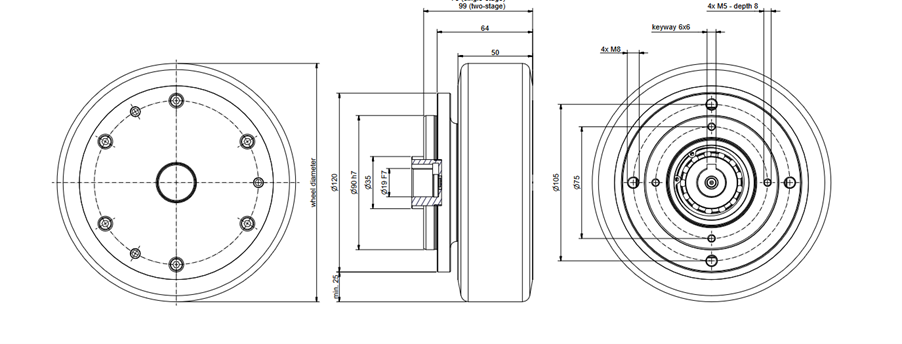
\includegraphics[width=\textwidth]{img/Picture1.png}
  \caption{drawing of the wheel}
  \label{wheel}
\end{figure}

where you can see(\cref{wheel}), in the bearings .The central component is the wheel, which comes in different diameters to facilitate movement by making contact with the ground. Encased within the wheel is the integrated planetary gearbox, designed to deliver high torque and precise speed control through multiple stages of planetary gears. The bearing supports this setup, ensuring the wheel rotates smoothly and steadily. Additionally, the mounting bracket, although optional, provides a secure means to attach the wheel drive to the robot or vehicle.
\begin{table}[h!]
  \centering
  \begin{tabular}{|l|c|}
      \hline
      \textbf{Parameter} & \textbf{Value} \\ \hline
      Wheel Diameter & $120 \, \mathrm{mm}$ \\ \hline
      Height & $125 \, \mathrm{mm}$ \\ \hline
      Load Capacity & $400 \, \mathrm{kg}$ \\ \hline
      Efficiency & $94 \%$ \\ \hline
      Max. Output Torque & $40.54 \, \mathrm{Nm}$ \\ \hline
      Mounting Bracket & Yes \\ \hline
      Weight & $4.8 \, \mathrm{kg}$ \\ \hline
  \end{tabular}
  \caption{Specifications of the Wheel}
  \label{tab:wheel-specs}
\end{table}

  \subsection{What is a mounting of an AGV?}
  The mounting of an Automated Guided Vehicle (AGV) involves securely attaching the AGV to a conveyor, docking station, or other transportation systems within a facility to ensure smooth and safe movement of goods or materials. These mounting devices are versatile, easy to install, and adjustable to fit various AGV sizes, often featuring quick-release mechanisms for efficient mounting and dismounting. By stabilizing the AGV during transportation, these devices minimize the risk of damage or accidents, thereby optimizing the AGV's performance and safety. Proper AGV mounting is crucial for seamless integration with other systems and enhancing overall productivity in industrial settings.
\begin{figure}[h!]
\centering
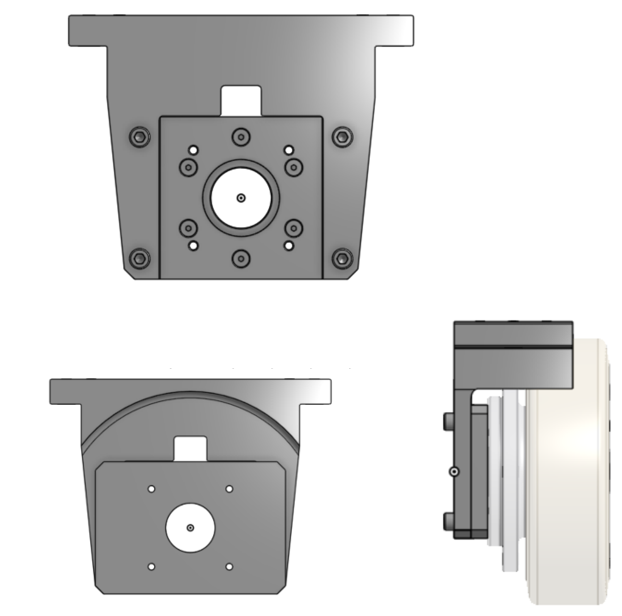
\includegraphics[width=\textwidth]{img/wheel3d.png}
\caption{}
\end{figure}

\subsection{Nanotec WD Wheel Drive and Hub gear NG500}

The Nanotec WD Wheel Drive and the Hub Gear NG500 both offer robust solutions for different applications, but they have their unique pros and cons. The Nanotec WD Wheel Drive stands out for its modular design, allowing for easy integration of various components like motors, brakes, and encoders, making it highly versatile and suitable for service robots and AGVs. Its availability in different wheel diameters also adds to its flexibility. However, it may not be the best choice for extremely heavy-duty applications due to its lower load capacity compared to the NG500. On the other hand, the Hub Gear NG500 excels in handling higher loads, up to $500 \, \mathrm{kg}$ per wheel, making it ideal for industrial applications like high-bay warehouses and automated agriculture. Its compact design and long service life, attributed to the separation of the gear and impeller, are significant advantages. However, its fixed wheel size might limit its adaptability to different use cases, and it may be less modular compared to the Nanotec WD Wheel Drive. In essence, the choice between these two depends on the specific requirements of the application, with the WD Wheel Drive being more versatile for robotics and the NG500 better suited for heavy-duty industrial needs.

\subsection{How is the Wheel Drive Attached to the Chassis?}
The mounting bracket has designated attachment points that align with corresponding points on the chassis. These points are typically threaded holes or slots that allow for bolts or screws to be used to secure the bracket to the chassis. Using appropriate bolts or screws, the mounting bracket is fastened to the chassis. It's important to use the correct type and size of fasteners to ensure a secure attachment. The bolts or screws are tightened to the specified torque to prevent loosening during operation.

Proper alignment of the wheel drive is crucial for optimal performance. The mounting bracket and attachment points are designed to ensure that the wheel is aligned correctly with the chassis, preventing any misalignment issues that could affect the movement and operation of the AGV. Once the wheel drive is securely mounted, the necessary cabling for the motor and encoder is connected.

\subsection{Benefits of the Mounting Design}
The modular design of this mounting system offers unparalleled versatility, allowing for easy integration into various robotics platforms and making it suitable for a wide range of applications. The stable and secure attachment provided by the mounting bracket prevents any movement or vibrations that could affect performance, ensuring reliable operation. Additionally, the minimized cabling effort and straightforward attachment process make installation quick and efficient, significantly reducing downtime and maintenance costs. The system's ability to combine with different motors, brakes, and encoders allows for extensive customization based on specific application requirements, enhancing its adaptability and functionality.

\section{THE CASTER WHEEL AND ITS COMPONENTS}

\begin{figure}[h!]
  \centering
  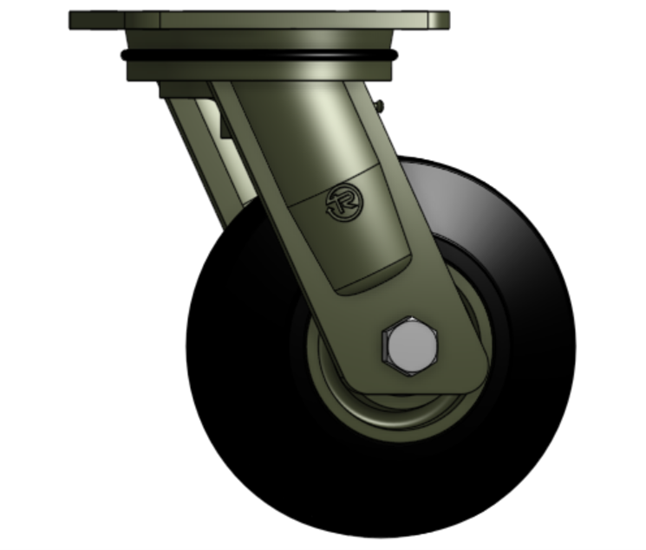
\includegraphics[width=0.5\textwidth]{img/caster.png}
  \caption[Key Components of a Caster Wheel]{A caster wheel consists of several key components that work together to provide smooth and efficient mobility}

  \end{figure}

\subsection{Wheel:}
This is the most visible part of the caster and is responsible for making contact with the ground. Wheels can be made from various materials such as rubber, polyurethane, nylon, phenolic, or cast iron, depending on the specific application and load requirements. Each material offers different benefits, like rubber providing a softer ride and cast iron offering high durability for heavy loads.

\subsection{Mounting System}
The mounting system connects the caster to the object it supports. There are two primary types: plate mounts and stem mounts. Plate mounts are used for heavier loads and provide a stable, secure attachment, while stem mounts are suitable for lighter applications where ease of installation is a priority.

\subsection{Swivel Mechanism}
This component allows the wheel to rotate 360 degrees, enhancing maneuverability. The swivel mechanism typically includes a raceway with ball bearings, which reduces friction and enables smooth, effortless swiveling. This is crucial for applications where tight turns and easy direction changes are necessary.

\subsection{Rigid Frame}
A fixed frame restricts the movement of the caster wheel to straight lines. This provides stability and control, making it ideal for applications where directional stability is essential, such as in straight-line travel paths.

\subsection{Brake System}
The brake system ensures that the caster stays stationary when needed. There are different types of brakes available, including wheel brakes that lock the wheel itself and swivel locks that prevent the swivel mechanism from turning. This added control is important for safety and precision in various applications.

\subsection{Bearing}
Bearings are installed inside the wheel hub or swivel mechanism to reduce friction and enable smooth rolling or swiveling. These components are critical for the efficient operation of the caster, as they ensure smooth, easy movement and reduce wear on the other parts.

\subsection{Axle}
The axle secures the wheel to the caster frame and ensures stability and alignment. It acts as a pivot point around which the wheel rotates and is usually made from durable materials to withstand the forces exerted during movement.

\begin{figure}[h!]
  \centering
  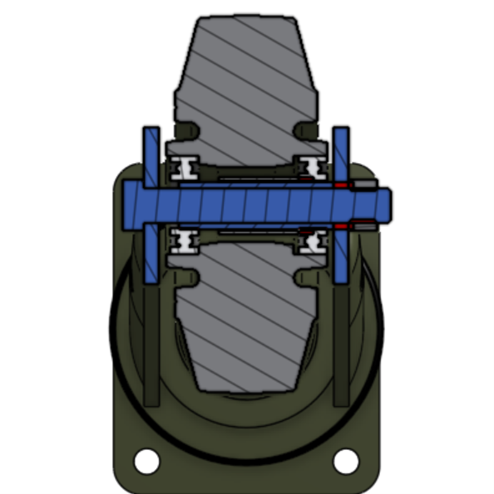
\includegraphics[width=0.5\textwidth]{img/Picture3.png}
  \caption{}
  \end{figure}

  Together, these components create a caster wheel that provides reliable, smooth mobility for a wide range of applications, from furniture and medical equipment to industrial machinery and warehouse carts. The careful design and selection of each component ensure that the caster meets the specific needs of its intended use, providing both efficiency and durability.

  \subsection{What is a Deep Groove Ball Bearing?}
A deep groove ball bearing is a widely popular type of rolling-element bearing, cherished for its versatility and efficiency. It consists of an inner ring, an outer ring, a cage, and a set of balls arranged in a circular pattern. The raceway grooves in both the inner and outer rings form a circular arc with a radius slightly larger than that of the balls, ensuring smooth and efficient rotation. 

These bearings stand out for their high load capacity, supporting both radial and axial loads, making them suitable for a wide range of applications. They also have low frictional torque, enabling high rotational speeds and reduced energy consumption. Their simple and compact design allows for easy installation and minimal space requirements. Furthermore, they are optimized for low noise and vibration, making them ideal for applications where quiet operation is essential.

Available in single-row and double-row designs, as well as open, sealed, and shielded variants, deep groove ball bearings can be customized to meet specific application needs.

\subsection{How Will the Inclination Be Handled?}
\begin{figure}[h!]
  \centering
  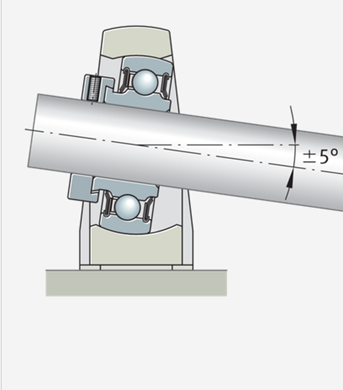
\includegraphics[width=0.4\textwidth]{img/Picture4.png}
  \caption{}
  \end{figure}

  Bearings with a spherical outer ring are designed to fit into housings with a concave bore, allowing them to compensate for any static misalignment of the shaft. This clever design ensures that even if the shaft isn't perfectly aligned, the bearing can still function smoothly.

However, there are limits to how much misalignment these bearings can handle. For maintenance-free housing units, the permissible angle of misalignment is $\pm 5^\circ$. For housing units with a relubrication facility, the allowable misalignment angle is $\pm 2.5^\circ$.

It's important to ensure that the center axes of the inner rings align on a straight line to achieve the best performance. This alignment ensures that the bearing operates efficiently and reduces the risk of premature wear or failure. This design is particularly useful in applications where maintaining perfect alignment is challenging, providing flexibility and reliability in various mechanical systems.

\section{Load carrying capacity}
\begin{figure}[h!]
  \centering
  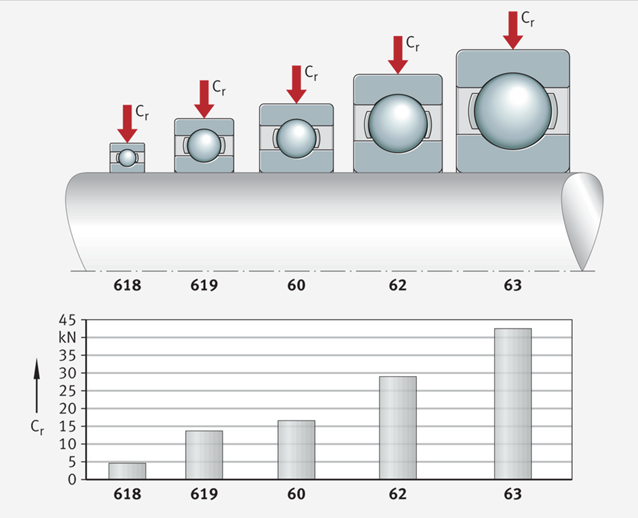
\includegraphics[width=\textwidth]{img/Picture5.png}
  \caption{}
  \end{figure}

\subsection{Suitable for Very High Radial Loads}
In radial insert ball bearings, the balls only make contact with the raceways at a single point. When the bearing is subjected to a purely radial load, these contact points lie at the center of the raceway. This means that the connection between the contact points passes directly through the radial plane, making the optimal load direction a purely radial one. Thanks to this design, radial insert ball bearings can support very high radial loads.

\subsection{Larger Ball Sets Permit Higher Loads}

The load-carrying capacity of a bearing depends on the bearing series and the size of the ball set within the reference bearings. For example, deep groove ball bearing series 60, which has a smaller bearing cross-section, cannot support loads as high as those of the standard series 62 of the same dimensions (relative to the bore diameter d), which features a larger ball set. If even higher loads are required for the same bore diameter, the heavy bearing series 63, with the largest ball set, is the best choice.
In summary, the design and size of the ball sets in radial insert ball bearings determine their ability to handle high radial loads, making them ideal for applications where such loads are present. This ability to support higher loads with larger ball sets ensures reliability and efficiency in a wide range of mechanical systems.



\section{Engineering Procedure}

\subsection{Bearing selection}

\subsubsection{Inputs and Assumptions}

\begin{enumerate}
\def\labelenumi{\arabic{enumi}.}
\item
  Wheel radius (R): 110 mm
\item
  Load on the wheel (F): 981 N
\item
  Maximum speed (v): 1.25 m/s
\item
  Shaft material: Steel (e.g., AISI 1045)

  \begin{itemize}
  \item
    Yield strength: $\sigma$y=250 MPa
  \end{itemize}
\item
  Bearing material: Chrome steel (e.g., AISI 52100)
\item
  Bearings catalog: We\textquotesingle ll pick based on
  calculated load and RPM.
\item
  Factor of safety (FOS): 2.0 for shaft design.
\end{enumerate}

\subsubsection{ Shaft Diameter Calculation}

\paragraph{Angular Velocity}
Convert the speed into angular velocity ($\omega$) to determine the RPM.
\begin{equation}
\omega = \frac{v}{R}
\label{eq1} 
\end{equation}

Substitute values in \cref{eq1}:

$$\omega = \frac{1.25}{0.06} = 20.83  \ \text{rad/s}$$

Convert $\omega$ to RPM:

$$ RPM = \omega \times 60/2\pi = 20.83 \times 60/2\pi \approx 199 \  \text{RPM}$$

\paragraph{Bending Moment and Shaft Diameter}

For a wheel shaft, the critical load is the bending moment due to the
force F. Assuming a simple beam supported at the bearing points:
\begin{equation}
  M = F \times L
\label{eq2}
\end{equation}

Where L is the distance from the bearing to the load. Assume
L=50 mm=0.05 \\m( minimum according to the ISO 3691-4:2020 standard):

$$ M = 981 \times 0.05 = 49.05\, \text{Nm}$$

Using the \textbf{maximum shear stress theory} for a solid circular
shaft, the shaft diameter is calculated from:
\begin{equation}  
 d = (16M/\pi\tau max)^{1/3} 
 \label{eq3}
\end{equation}

Where:

\begin{itemize}
\item
  \(\tau max\): Allowable shear stress =
  \(\sigma y/2 \times FOS = 250/2 \times 2 = 62.5\, MPa = 62.5 \times 106\, Pa\)
\end{itemize}

Substitute values in \cref{eq3}:

\(d = (16 \times 49.05/\pi \times 62.5 \times 106)^{1/3}\)= 0.012mm

\subsubsection{Bearing Selection}

\paragraph{ Load on the Bearing}

The radial load on the bearing is equal to the load on the wheel:
$$Fr = 981\, \text{N}$$

\paragraph{Dynamic Load Rating}

Using the bearing life equation:

$$C = Fr \times (L/1,000,00{0)}^{\frac{1}{3}}$$
Where:

\begin{itemize}
\item
  L: Bearing life in revolutions. Assume L=\(10^{6}\) revolutions.
\end{itemize}

\(C = 981 \times (10^{6}/1,000,000)^{1/3} = 981\, N\)

From a standard bearing catalog, a \textbf{deep groove ball bearing}
with a dynamic load rating C\textgreater981 N and an inner diameter
matching the shaft size (d=12 mm) is selected:

\begin{itemize}
\item
  \textbf{Bearing Type:} Deep groove ball bearing (e.g., 6201 series).
\item
  \textbf{Verification :}
\end{itemize}

\subsubsection{Material Properties of AISI 1045 Steel}

\textbf{Yield Strength (}$\sigma$y\textbf{)}: Approximately 530 MPa

\textbf{Ultimate Tensile Strength (}$\sigma$u\textbf{)}: Approximately 625 MPa

\subsubsection{Calculation}

\begin{enumerate}
\def\labelenumi{\arabic{enumi}.}
\item
  \textbf{Cross-Sectional Area (A)}:
\end{enumerate}


$$A=\pi\left(\frac{d}{2}\right)^2=\pi\left(\frac{12\, \text{mm}}{2}\right)^2 \approx 113.1\, \text{mm}^2$$

\begin{enumerate}
\def\labelenumi{\arabic{enumi}.}
\setcounter{enumi}{1}
\item
  \textbf{Stress (}$\sigma$\textbf{)}:
\end{enumerate}


A shaft of 12mm diameter made of AISI 1045 steel can safely bear a load of 981N, as the induced stress is well within the material's yield and ultimate tensile strengths.
$$
\sigma = \frac{F}{A} = \frac{981 \text{ N}}{113.1 \text{ mm}^2} \approx 8.67 \text{ MPa}
$$

\paragraph{3.3 Number of Balls in the Bearing}

To determine the diameter of the balls in the bearing when we are
supposed to have 9 balls( i tried all the number less than 9 , they were
not compatible with the standard), we can use the following formula:
\begin{equation}
  \text{z} = \frac{\pi (D + d)}{2 d_b}
  \label{eq4}
\end{equation}

where: $z$, the number of balls; $D$, the outer diameter of the bearing; $d$, the inner diameter of the bearing; and $db$, the diameter of each ball. For this specific case, the given values are as follows: $z = 9$, $D = 32 \, \mathrm{mm}$, and $d = 12 \, \mathrm{mm}$.

We need to solve for db:
\begin{align*}
  z &= \frac{\pi (D + d)}{2 db} \\
  9 &= \frac{\pi (32 + 12)}{2 db} \\
  9 &= \frac{\pi \cdot 44}{2 db} \\
  db &= \frac{\pi \cdot 44}{2 \cdot 9} \\
  db &\approx 7.68 \, \mathrm{mm}
\end{align*}

For a 6201 bearing:

\begin{itemize}
\item
  Number of balls: Typically 7--9 balls.
\item
  Ball diameter: beyond 4.5 mm.
\end{itemize}

\subsubsection{Material Selection}
\paragraph{Shaft Material: AISI 1045 Steel}

\begin{itemize}
\item
  Reason: High strength, good machinability, and readily available.
\end{itemize}

\paragraph{Bearing Material: AISI 52100 Chrome Steel}

\begin{itemize}
\item
  Reason: High hardness, wear resistance, and durability under dynamic
  loads.
\end{itemize}

\subsubsection{Compatibility Check}

A deep groove ball bearing that meets these specifications is the
\textbf{NSK 6201} bearing. Here are the details:

\begin{itemize}
\item
  \textbf{Inner Diameter (ID)}: 12 mm
\item
  \textbf{Outer Diameter (OD)}: 32 mm
\item
  \textbf{Width (W)}: 10 mm
\item
  \textbf{Material}: AISI 52100 Chrome Steel
\item
  \textbf{Load Capacity}: Suitable for the given load and speed
  requirements
\end{itemize}

\newpage
\begin{figure}[H]
\centering
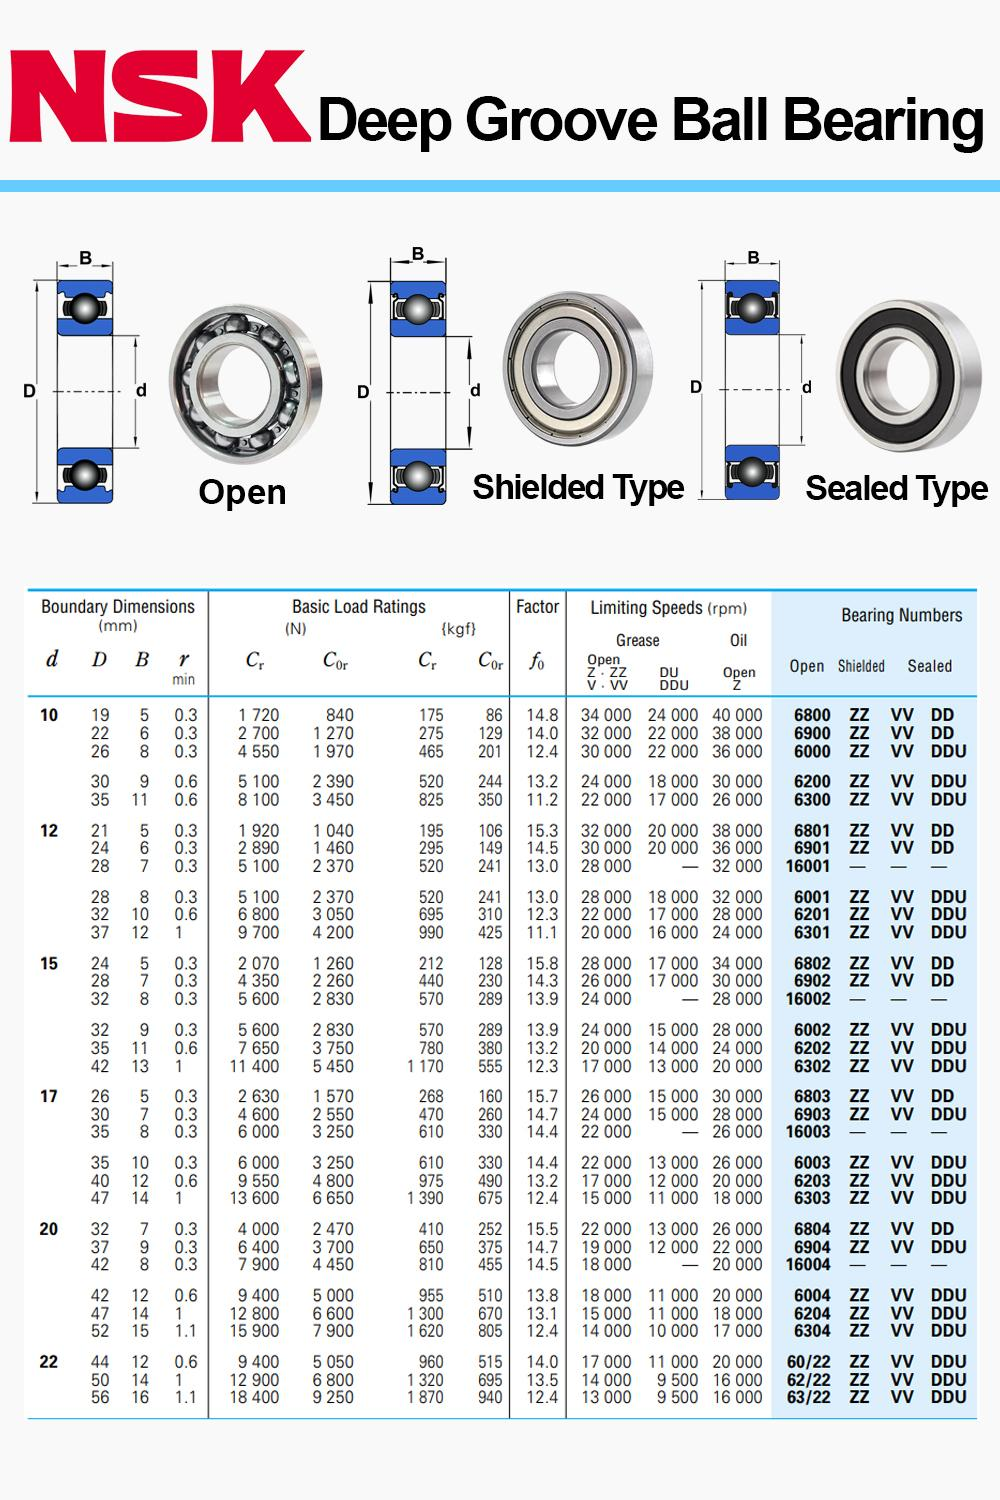
\includegraphics[width=\textwidth]{img/img1.jpg}
\caption{}
\end{figure}
\newpage

\subsection{Torque calculation}

\subsubsection{Given Data:}
\begin{itemize}
\item
  Gross Vehicle Weight: 300 kg
\item
  Weight per Drive Wheel: 100 kg
\item
  Maximum Incline Angle: 8°
\item
  Maximum Velocity: 1.5 m/s
\item
  Surface: Concrete
\item
  Type of Bearing: Deep Groove Ball Bearing (NSK 6201)
\item
  Wheel Type: Rubber Tires
\item
  Drive Wheel Diameter: 95 mm (0.095 m)
\end{itemize}

\subsubsection{Load Analysis:}
\begin{enumerate}
\def\labelenumi{\arabic{enumi}.}
\item
  \textbf{Load Calculation}:
  
  \(F = W = 100\, kg \times 9.81\, m/s2 = 981\, N\)
  
  \item
  \textbf{Wheel Rotational Speed}:
  
  \(r = 0.22\, m/2 = 0.11\, m\)
  
  \(Circumference = \pi \times d = \pi \times 0.22\, m = 0.6909\, m\)
  
  Wheel Rotational Speed=Linear Speed
  
  \(Circumference = 1.25\, m/s\ /\ 0.6909\, m \approx 1.81\, r/s \approx 108.6\, RPM\)
  

\item
  \textbf{Required Torque}:

\(T = F \times r = 981\, N \times 0.11\, m = 107.91\, Nm\)

Considering efficiency and safety:

\(Efficiency(85\%),Tmotor = Tt/Eff. = 107.91\, Nm/0.85 = 126.95\, Nm\)

(without bearing)
\item
\textbf{Torque Required for Acceleration}: Assuming $\alpha$=1m/s\^{}2:

Require Tractive effort (Ft)

\(Ft = mt\ x\ \alpha = \ 300\ kg\ x\ 1\ m/s^{2} = 300N\)

Force must be provided by frictional force at the wheel

\(T = Ft\ x\ r = 300N\ x\ 0.11m = 33\, Nm\)

\item
  \textbf{Effect of Inclination}:

\(\theta = 3{^\circ} = 0.0524\, rad\)

\(Gravity\ Component = 300 \times 9.81 \times sin(0.0524) \approx 154.11\, N\)

\(Tincline = \ Fgravity\ x\ r = 154.11N\ x\ 0.11m = 16.9521\, Nm\,\)

\item
  \textbf{Torque Due to Friction}: Assuming $\mu$=0.002(coef.
  friction):16.9521 Nm
\end{enumerate}

\(Ffriction = \mu\ x\ R\  = \ 0.002\ x\ 981N = 1.962N\) (R: radial load)

\(Torque\ Due\ to\ Friction = Ff \times r = 1.962\, N \times 0.006\, m = 0.011772\, Nm\)
(r=bore radius)
\\ \\
\textbf{Total Torque Required}:

\(Ttotal = T1 + Tfriction = 33\, Nm + 0.011772\, Nm = 33.211772\, Nm\)

\textbf{Verification:}

\begin{itemize}
\item
  The NSK 6201 bearing has a basic dynamic load rating of 7.28 kN, which
  is sufficient to handle the load of 981 N.
\item
  The calculated torque values and rotational speed are within the
  bearing\textquotesingle s specifications.
\end{itemize}

\subsection{Results}

The outcomes of the computations and validation procedures are as
follows:

\subsubsection{Shaft Measurements}

12 mm is the calculated shaft diameter.

Approximately 8.67 MPa of induced stress is much less than the
material\textquotesingle s \\ yield strength of 250 MPa.

\subsubsection{Bearing Details:}
NSK 6201 deep groove ball bearing model.

Dimensions:

- 12 mm in diameter within.

- 32 mm in diameter outside.

- Capacity to load: Equipped to manage loads that are above the
designated 981 N.

- Ball diameter: 7.68 mm, which meets catalog requirements for nine
balls.

\subsubsection{Observance of Standards}
By following ISO 3691-4:2020 guidelines, the design guarantees
load-handling systems\textquotesingle{} dependability and safety. For
operating performance, the shaft and bearing dimensions meet the minimal
requirements.

\subsubsection{Total Torque Required:}

The dynamic load needed is 28.2Nm


\end{document}